\subsection{HSPからJuliusを使う}
認識した音声を元に何か処理を行いたいことはしばしばあります。例えば、認識した音声に応じて部屋の電気をつけたり、タイマーをセットしたりということが考えられます。そんなときには自分のプログラムと連携させましょう。
\subsubsection{JuliusとHSPの連携のしくみ}
Juliusは図\ref{JuliusとHSPの連携}のように、HSPの外で動きます。別に起動しているJuliusと、書いたHSPプログラムが「ソケット」と呼ばれる通信経路を介して通信することで認識結果やコマンド(Juliusの起動・停止など)のやり取りをすることができます。
\begin{figure}[H]
\begin{center}
    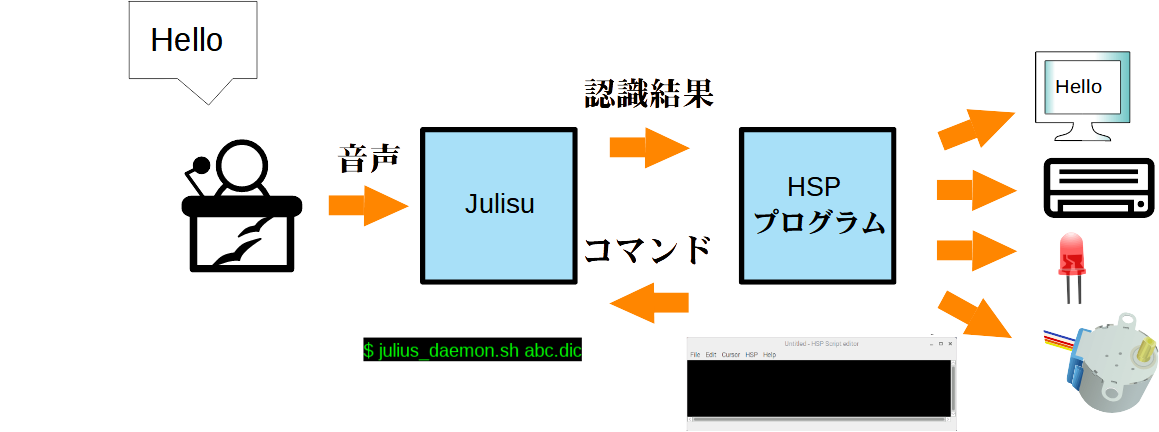
\includegraphics[width=\linewidth]{images/chap06/text06-img010.png}
    \caption{JuliusとHSPの連携}
    \label{JuliusとHSPの連携}
\end{center}
\end{figure}
従って、HSPからJuliusを使うためには、HSPプログラムだけではなく別にJuliusも事前に起動させておかなければなりません。

\subsubsection{認識した単語を取得・表示する}
新しく覚える命令と関数は\code{init\_julius},\code{is\_recieved()}, \code{get\_word\_list} の3つです。例題のプログラム julius.hsp を見ながら解説していきます。\\
\begin{lstlisting}[caption=julius.hsp,label=julius.hsp]
#include "hsp3dish.as"
#include "julius.as"

redraw 0
pos 0, 0
mes "Loading Julius..."
redraw 1

init_julius "/home/pi/ome/06/kudamono.dic"

sockidx = 0
domain = "127.0.0.1"
PORT = 10500

sockopen sockidx, domain, PORT

if stat != 0 {
*errorjulius
  redraw 0
  pos 0, 0
  mes "Error in opening socket"
  redraw 1
  await 30
  goto *errorjulius
  stop
}

sdim words, 4096, 0
ddim cm, 0

repeat -1
  if is_recieved(sockidx) == 0 {
    get_word_list words, cm
    len =  "L1 " + length(words)
    repeat length(words)
      if cm(cnt) > 0.5 {
          ans =  "" + cnt + ": " + words(cnt) + " CM = " + cm(cnt)
      }
    loop
  }
  redraw 0
  pos 0,0
  mes len
  mes ans
  redraw 1
  await 30
loop
\end{lstlisting}
まず、\code{init\_julius},\code{is\_recieved}と\code{get\_word\_list}を使えるようにするために、2行目のように\\
\code{\#include “julius.as”}
を書きます。

続いて、\code{init\_julius}を実行してjuliusを使うための初期化 (initialization) を行います。これは\code{is\_recieved}と\code{get\_word\_list}が実行される前に一回だけ実行されるよう書く必要があります。これによってJuliusが起動します。引数には使用する辞書ファイル (今回は/home/pi/ome/06/kudamono.dic) を指定してください。続いて、\code{sockopen}命令でjuliusと通信するための経路 の番号(ソケットIDと呼びます) を\code{sockidx}、つまり0に設定します。juliusは自分のラズベリーパイ (127.0.0.1) の10500番ポートを使用します。このとき、エラーが起きればシステム変数\code{stat}に0以外の値が入るので、statに0以外の値が入っていたらエラーメッセージを表示して終了する条件分岐を書きます。

続いて、\\
\code{sdim words, 4096, 0\\
ddim cm, 0}
は、juliusの認識結果を格納するための配列を宣言しています。juliusは認識結果として2つの要素を出力します: 1つめは認識された単語、2つ目は認識の正確さ(単語信頼度)です。それぞれが文字列配列\code{word}と小数配列\code{cm}に格納されます。認識された単語が必要なのはもっともですね。単語信頼度は、juliusがその認識結果にどれだけ自信があるかを示します。1が最大(最も自信がある)で0が最小(最も自信がない)で、小数で表されます。\\
\code{repeat -1}
以下が認識結果を画面に表示するための無限ループによるメインルーチンになります。is\_recieved(sockidx)は、sockidxの先のjuliusから認識結果を取得し終えたら0が帰ってきます。従って、0が返ってきたときだけ認識結果の代入と画面表示の処理を行うように条件分岐が書いてあります。\\
\code{get\_word\_list word, cm}
によって、文字列配列wordと小数配列cmに認識結果が代入されます。wordとcmは配列なので、次のrepeat文でそれぞれの要素に対して、cm(単語信頼度)が0.5以上のもののみmes命令を実行し、結果を画面に表示させています。\\
\begin{tcolorbox}[title=\useOmetoi]
\begin{enumerate}
\item HSPでjulius.hspを実行しましょう。\\果物の名前を3つ話しかけて、認識されるか確かめてみましょう。\\□←できたらチェックしましょう。
\end{enumerate}
\end{tcolorbox}